\documentclass[review]{siamart190516}
\usepackage{amsmath,amssymb,eucal,graphicx}
\usepackage{amsthm,wrapfig,float,adjustbox}
\usepackage{hyperref}
\usepackage{booktabs}
\usepackage{xurl}
\usepackage{caption, subcaption}

\title{Bayesian Neural Networks\thanks{RSCAM Group Project,
Supervisor: Benedict Leimkuhler}}
\author{Lukas Peham
\and Andy Grant
\and Uday Singh
\and Hari Madhukumar
}

\renewcommand{\baselinestretch}{1.5}

\begin{document}

\maketitle

\begin{abstract}
    This project focuses on a Bayesian approach to neural networks and the extra information they can convey when compared to the frequentist approach. We use primitive data sets to create our Bayesian model and form a numerical estimate for the posterior distribution via the Metropolis-Hastings, Monte-Carlo Markov chains method. The resultant posterior distributions display the success expected from parameters across a range of values in a given network for a simple classification task. We use these distributions to show why gradient descent based methods can be problematic when there is multi-modal behaviour exhibited. Furthermore, we use Bayesian model averaging to evaluate the posterior distribution and then retrain the network with the knowledge gained. 

\end{abstract}

\section{Introduction} \label{sec:intro}

Artificial neural networks mimic the human brain in that they allow the computer to learn from ‘experience’. Real world data is interpreted in terms of features which are arranged in hierarchies, each feature defined through its relation to simpler characteristics [5]. This process is called deep learning as the hierarchy comprises layers upon layers of features.
\newline 
The standard procedure involves feeding a machine learning algorithm a set of training data through the visible layer (input). The neural network utilises its hidden layers to extract a variety of features from this raw data, such as pixel density, brightness etc., in the case of image data. Since the correct answers are known for the training data, the neural network can improve its perception by tweaking the weights it assigns to each feature in each layer, and finally, in the output. The error in the output is measured by a Loss function, which can take many forms, of which squared error loss is one:
\begin{equation} \label{eq:loss}
\mathcal{L}(w) = \min_{w} \Sigma (f (x_i; w) - y_i)^2.
\end{equation}
Optimisation algorithms help minimise this loss by finding minima in the parameter space be employing methods such as Gradient Descent (SGD,ADAM, etc.). The objective is to find minima which have a low generalisation error. Networks with a low generalisation error perform similarly on test data as training data and will not over fit to the training data.
Thus, using these parameters obtained from gradient descent we have a neural network which can be employed for real world tasks, such as programming driver-less cars or diagnosing Alzheimer's where even human experts fail \cite{OZSAHIN2020183}. 
\newline 
In applications such as these, the margin of error is very low \cite{indrayan2008medical}, as the stakes are very high. A traditional neural network will train its parameters and then produce point estimates as the predictions. In other words, the weights that are trained in the network correspond to a local minima of the loss function.
\newline 
In this report we start with a general comparison of the Bayesian and frequentist approaches to neural networks followed by a discussion on generalisation uncertainty. Then we move on to produce.....

\section{Bayesian vs frequentist} \label{sec:bayes_freq}
Now let's discuss the differences and also similarities between Bayesian and frequentist neural networks. In order to start this discussion we briefly need to talk about the types of uncertainties that can arise from model predictions.
Epistemic uncertainty arises due to limited data or knowledge (provided to the model). Increasing training samples should cause epistemic uncertainty to decrease. Any neural network model would be vulnerable to Epistemic uncertainty, and a model that seems to fit too well despite this, is probably over-fitting and would not generalise well. \newline
Aleatoric uncertainty stems from stochastic noise present in observations, and other random errors such as errors in measurement \cite{yarin2016uncertainty}.
In cases such as these, where the uncertainty is high, a standard neural network would output a point estimate regardless. However, a Bayesian network would return a posterior which we could use to construct a credible interval as a measure of the uncertainty. This is important in fields like medicine, where a surgeon isn’t concerned solely with the accuracy of a prediction (classification) but also the uncertainty inherent in the prediction. 
\newline 
Another advantage Bayesian neural networks have over traditional neural networks is that optimisation algorithms are not always reliable \cite{reliablitiy}. There is also an uncertainty associated with the training of parameters. In traditional gradient descent, the parameters are trained to minimise the loss without a full exploration of the loss landscape. There is no guarantee that an optimiser based on stochastic gradient descent finds a global minimum.
\newline 
The Bayesian approach allows us to generate posterior distributions for the parameters, using our priors (informed or vague) and the likelihood of the observations. We can then examine this posterior to analyse the loss landscape. This analysis can involve identifying whether a posterior is multi-modal and how wide or narrow the support of the modes are. The width of the support is indicative of the \textit{shape} of a minima which in turn influences the generalisation error. In the frequentist approach the the sought after parameter values is the  MAP (\textit{Maximum a Posteriori}) estimate of the posterior. However, this is not always the most desirable parameter value to find. We discuss this further in section \ref{sec:gen_error}.
It is frequently found that for a well trained network, at least one of the modes of the posterior will lie on the maximum likelihood estimate produced by the optimiser. 
\newline 
This gives a posterior distribution for the parameters and maximum likelihood estimate gained from standard training or MAP estimate via analysing the posterior. However, we know that it is not advised to rely on point estimates and ignore inherent uncertainties when the model needs to be applied in high risk situations. Thus, the next step is to obtain a predictive distribution,
\begin{equation}
     p(y|D,x) = \int p(y|w,x) p(w|D) dw.
\end{equation}
Here, $y$ is the new data to be predicted, $w$ are the set of optimised parameters and $D$ is the training data we used to train the parameters. We are essentially integrating over the marginal likelihood of the weights. This method is known as Bayesian Model Averaging (BMA) with a fixed network architecture, taking the average over all possible models, where each parameter vector represents a different model. In order to do BMA with networks of different architecture one needs to further include priors for different models and combine it with the posteriors.

So far we have discussed how using a Bayesian approach might be more advantageous, now we will comment on some possible disadvantages. As we know, instead of providing us with point estimates for the parameters, a Bayesian network returns entire probability distributions. Since getting these distributions analytically, we require sampling techniques. We choose Markov Chain Monte Carlo techniques to produce these samples. These techniques use conditional densities for the weights instead of treating them all as independent. This is ideal for Bayesian inference. In particular, we used the popular Metropolis Hastings algorithm (to be described in detail in section \ref{sec:metro_hast}). A common technique to diagnose convergence is using Gelman-Rubin statistics.

However, aside from training the neural network, which can be a long and arduous task for large data sets with complex feature spaces, we also have to account for the time taken up by simulation. This time will also increase exponentially with the size of the model and it will computationally expensive to perform such a task. 
A simpler approach, would be to explore the posteriors of a smaller subset of weights, keeping the rest constant at their optimised levels, and retrain the network using MAP estimates from the posterior.

\section{Generalisation uncertainty} \label{sec:gen_error}
With a point estimate for the minimisation of the loss function you have no appreciation of what loss the surrounding points in the parameter landscape will achieve. Hence, it is hard to establish whether this point lies in a 'flat' minima or a sharp minima. As discussed in various literature \cite{Tom}, \cite{Sepp}, \cite{Nitish}, sharp minima tend not to generalise as well as flatter, bowl shaped minima. A point estimate obtained by some variant of stochastic gradient descent will not be able to discern the nature of the minima, thus possibly resulting in a high generalisation error which could potentially have calamitous consequences in industrial application as discussed in the introduction \ref{sec:intro}.

One proposed solution to this is to use a loss function which takes into account the loss value of surrounding points. Pratik Chaudhari et al.\cite{Pratik} incorporate the \textit{local entropy} into a loss function, 
\begin{equation}
\mathcal{L}(x) = \log \int_{x^{\prime}} \exp \left(-f\left(x^{\prime}\right)-\frac{\gamma}{2}\left\|x-x^{\prime}\right\|_{2}^{2}\right) d x^{\prime}.
\label{local entropy loss_function}
\end{equation}
This loss integrates over all points $x^{\prime}$ within a neighbourhood of $x$ in the parameter space. $\gamma$, or the \emph{scope}, is the parameter that varies the size of this neighbourhood and $f()$ is the standard loss function of equation \ref{eq:loss}.
This formulation of the loss function penalises points which lie in more volatile areas of the original loss landscape, hence giving more merit to flatter minima.

This approach to uncertainty in point estimates is beneficial yet still not anywhere near as informative as the Bayesian approach. In what follows we will find or approximate the Bayesian posterior distribution for some basic Neural networks in order to better analyse the parameter space.

\section{Neural network without a hidden layer} \label{proto_bnn}
To begin with we will outline the first Bayesian neural network (BNN) that we produced. In order to try attain a firm understanding of the fundamentals, we built up our first BNN from scratch. We made it as primitive as possible to aid interpretability with a plan to add complexity later.

\begin{wrapfigure}[10]{r}{0cm}
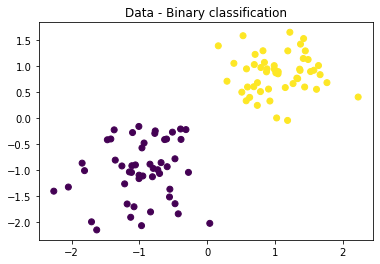
\includegraphics[scale=0.5]{Images/data1.png}
\caption{Data for simple classification task}
\label{fig:data}
\end{wrapfigure}

Our data consists of points in a 2d plane. We manufactured two groups of 50, one centered around $(-1,-1)$ (labelled 0) and the other around $(1,1)$ (labelled 1). The points follow a normal distribution (in both x and y) with a standard deviation of 0.5. The aim is to fit a line that separates the two groups. In the figure \ref{fig:data} we show this data which we will also use later on.


 The model consists of two inputs, x and y, that were fed into a function to calculate the distance of each data point from a proposed line $l$, $y=kx+d$, \ref{distance}. Each of these distances are fed into a sigmoid output function ($\sigma$) and the loss \ref{loss_1_hidden} was calculated from the difference between this classification and the true label:
 \begin{equation}
    dist(p_{i},l) = \frac{y_{i}-\left(k x_{i}+d\right)}{\sqrt{k^{2}+1}},
    \label{distance}
 \end{equation}
\begin{equation}
    \mathcal{L}(k,d|D) = \sum_{i=1}^{100}\left(  \sigma(dist(p_{i},l)) - C(p_{i}) \right)^{2}.
    \label{loss_1_hidden}
    \end{equation}
Above, $D$ represents the data set of 100 points and $C(p_{i})$ is the true classification label for point $p_{i}=(x_{i},y_{i})$ in the data set.
The resultant model is not strictly a neural network since it does not have any hidden nodes.
\newline
We then proceed to produce our likelihood function via exponentiation of the loss function,
\begin{equation}
    p(D|k,d)=e^{-\mathcal{L}(k,d|D)},
\end{equation}
which is evaluated on every point on a $(slope, bias) = (k,d)$ grid.
Using Bayes formula we combine this likelihood  with an appropriate prior (we arbitrarily chose two Gaussian priors for this illustrative example,) to form the posterior distribution :
\begin{figure}[h!]
    \centering
    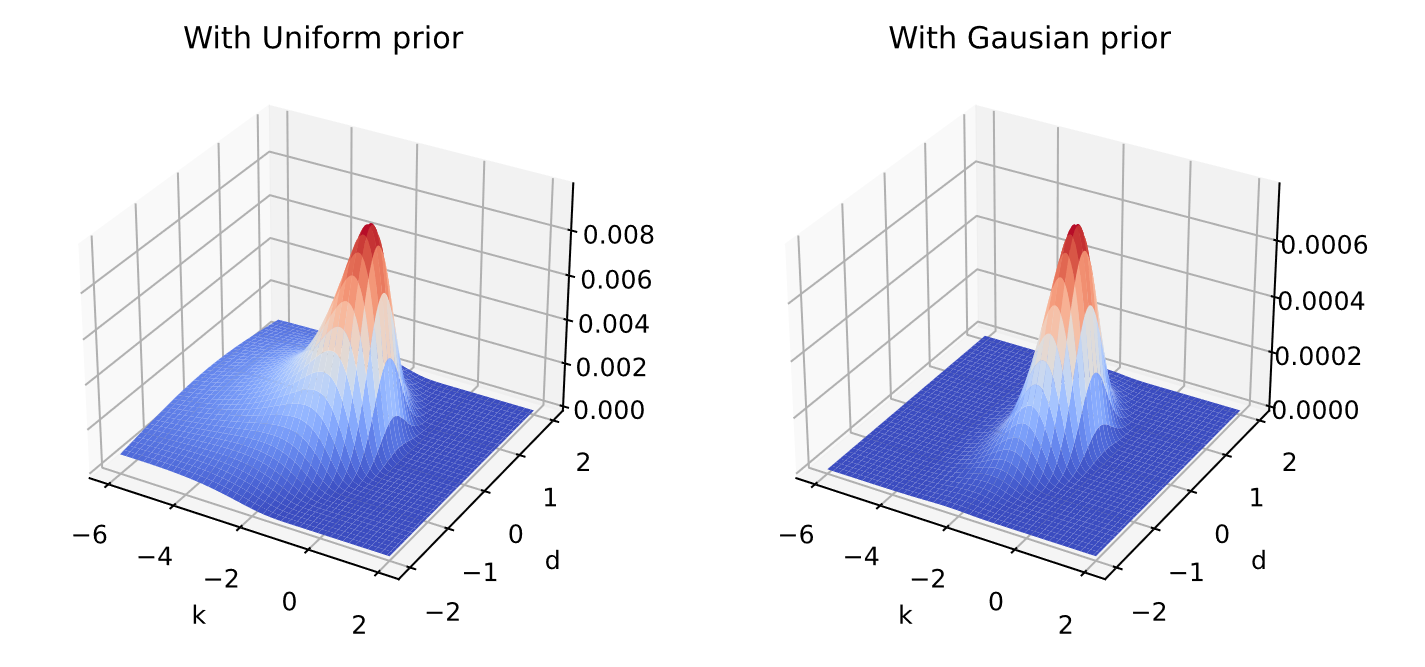
\includegraphics[width = \textwidth]{Images/posterior.png}
    \caption{Posterior of the prototype network}
    \label{fig:post}
\end{figure}
From these visualisations we can see how a whole distribution of parameter values compare at this classification task. Both posteriors display a zero probability density for positive slopes since this would give rise to separating lines which cut through both groups rather than separating them.
Also apparent is the effect of the prior on the posterior. The normal prior gives a sharper peak, indicating that a narrower range of parameter values will classify well on the data. Due to the simplicity of the problem the prior choice is not very important.
\newline Priors can be very useful for larger problems where some pre-existing knowledge is available. If there is a region of the parameter space in which it is known that the desired value exists then by using a prior with high density over this area, you can form a posterior which is biased towards these values. It is often also the case that large parameter values are less desirable and hence a prior can be used to bias a model towards smaller ones. Next we move onto add in complexity to our model with a hidden layer.

\section{Neural network with one hidden layer}
We initially continue with the same data set as the previous section but use a neural network with one hidden layer.
\newline
Otherwise the framework will be similar to the previous section with two inputs and a sigmoid output. This network will have two weights and a bias parameter for each node. There are 2 hidden nodes and one output node, hence we get 9 parameters in total. Clearly this is an over-parameterisation of a problem which only requires two parameters in reality. However, due to this over-parameterisation the neural network should find many different solutions to the same problem. This should in turn create more interesting posterior distributions with multiple modes with which we can use our Bayesian approach for a deeper analysis.
\subsection{Neural network implementation}
In order to be able to compare the Bayesian approach to the frequentist, we employed gradient descent to find a point estimate. Rather than use a black-box Python module we decided to implement back-propagation from scratch. This helped us gain a more intimate understanding with such structures.
\newline
Once we had our point estimate for a parameter value that optimised the network at the classification problem, we wanted to visualise how it handled the task. This would give us a tangible idea of how different parameter values in our 9-dimensional parameter space approached the task. For the initial data the point estimate obtained represented a straight line which classified the data very similarly to the maximum likelihood estimate of the posterior distribution in the previous section. To provoke the network into exhibiting non-linear behaviour, we increased the standard deviation of the $x$ and $y$ coordinates in the data to $1.5$.
\newline 
\begin{figure}[h!]
    \centering
    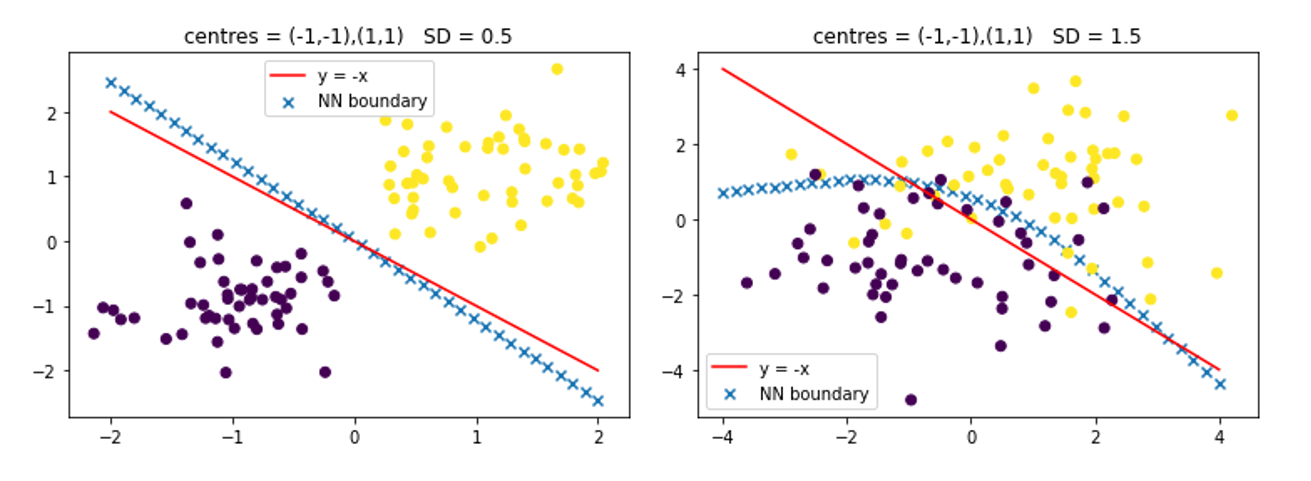
\includegraphics[width = \textwidth]{Images/1.png}
    \caption{NN with 1 hidden layer}
    \label{fig:1}
\end{figure}
In \ref{fig:1} you can see the boundary of the neural network. We calculated this by solving for when the sigmoid function output of the network gives $0.5$, i.e., when the model cannot pick between the two labels, $0$ and $1$. This was possible due to the relative simplicity of the network. For larger networks this is not feasible. Instead you can evaluate the network on a grid of input values to see how it classifies.
\newline
On the right hand side plot of \ref{fig:1} you can see some non-linear behaviour being exhibited by the network as it tries to deal with overlapping data.
\subsection{Circular data}
Next we increase the difficulty of the classification task. One of the groups in the new data consists of points normally distributed about $(0,0)$ with a standard deviation of $0.05$. The other group is sampled from a circle of radius $1$. We do this by first parameterising the circle and and picking parameter values randomly from a uniform distribution to give 50 points on the circle. Then we add in Gaussian noise in the $x$ and $y$ directions to each point with standard deviation of $0.05$. This produces plots as seen in \ref{fig:2} and \ref{fig:3}.
\newline
To begin with we trained our one layer model on only a semi-circle of data so not to make the classification task too hard, as seen in figure \ref{fig:2}. We then increase the standard deviation to $0.3$ and train the network again, illustrated in the right hand side of figure \ref{fig:2}. 
\begin{figure}[h!]
    \centering
    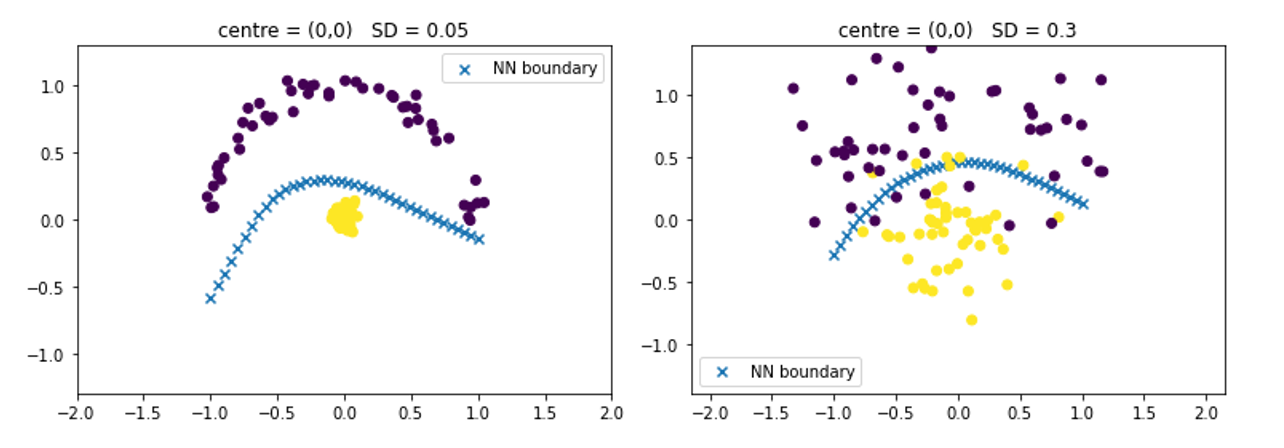
\includegraphics[width = \textwidth]{Images/2.png}
    \caption{NN with 1 hidden layer}
    \label{fig:2}
\end{figure}
\newline
The network performs very well in both instances, seemingly optimising the loss in both tasks. 
\newline 
Finally, we run gradient descent for the full circle of data. First for points with noise at a standard deviation of $0.05$ and then at $0.15$. Figure \ref{fig:3} clearly shows that the network is employing the same strategy to both tasks, which is not desirable. The desired strategy would involve a curved boundary rather than straight lines. The loss curves for these point estimates do not reach near zero as expected. Initially we believed that this lack of success was due to the simplicity of our model. Hence we added 2 more hidden layers. However this also resulted in similarly poor loss.
\begin{figure}[h!]
    \centering
    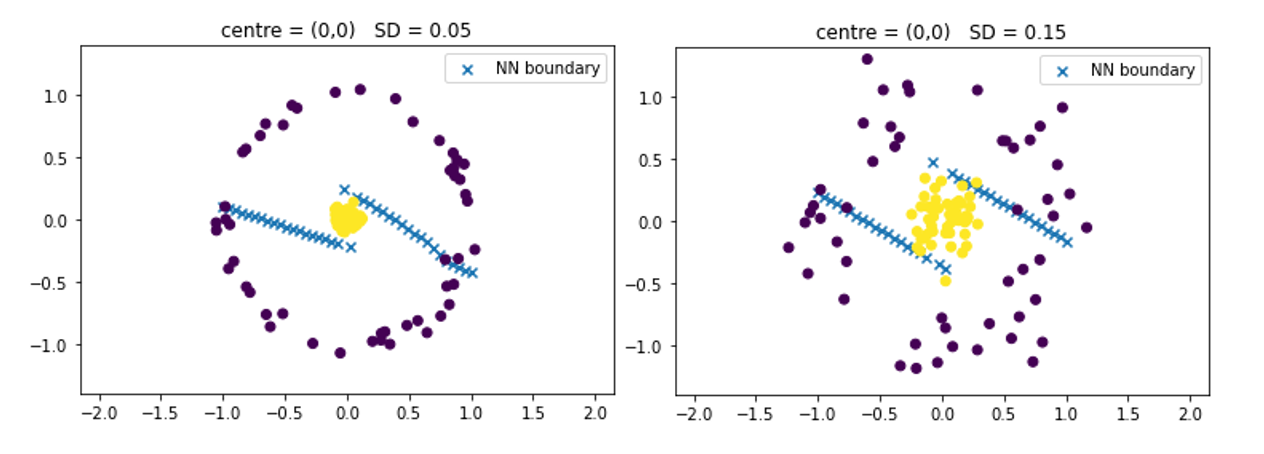
\includegraphics[width = \textwidth]{Images/3.png}
    \caption{NN with 1 hidden layer}
    \label{fig:3}
\end{figure}
\newline 
In the next section we will use numerical techniques to sample from the posterior distribution of networks created in this section in order to try discern why such models have trouble locating the desired minima. The aim is to use Bayesian techniques to assess the issues with gradient descent and then improve upon them.

\section{Sampling posterior of a neural network with one hidden layer}

The key distinguishing property of a Bayesian approach is to represent solutions given by all settings of parameters weighted by their posterior probabilities (marginalisation), rather than obtain a single set of parameters (optimization). To understand how marginalisation can make a big difference for accuracy and calibration, we study the marginal distributions of the parameters when training the neural network. This requires sampling from the posterior distribution.

\subsection{Markov Chain Monte Carlo (MCMC)} \label{sec:mcmc}
%stuff about mcmc methods

Markov Chain Monte Carlo is a sampling method that draws random samples from a desired distribution. In this case, the desired distribution will be the posterior distribution of parameters that we obtain from the neural network.

The samples are generated from a Markov Chain that converges to the posterior after a certain number of iterations excluding a burnin phase. Constructing the Markov chain that converges to the target distribution is the essence of MCMC. Generally, multiple chains are run with different initial values. A very popular MCMC algorithm is Metropolis Hastings, which we introduce next.

\subsection{Metropolis Hastings Algorithm} \label{sec:metro_hast}

In order to sample the posterior distribution, we first implemented the Random walk Metropolis-Hastings Algorithm. The Metropolis-Hastings algorithm is an iterative sampling procedure which generates a sequence $\theta_0,\theta_1,\theta_2,...,\theta_N$, where each $\theta$ represents a vector of parameters for the neural network under consideration. The steps involved in the algorithm are as follows:
\begin{itemize}
    \item \textbf{STEP 1:} Initialize a starting value $\theta_0$. 
    \item \textbf{STEP 2:} For the current state $\theta_c$, draw a proposal value $\theta_p$ from a Gaussian distribution $N(\theta_c,diag(1))$.
    \item \textbf{STEP 3:} Calculate probability of acceptance, which is the ratio of the posterior probabilities, $\alpha = \frac{\pi(\theta_p)\exp^{-\mathcal{L}(\theta_p)}}{\pi(\theta_c)\exp^{-\mathcal{L}(\theta_c)}}$, where $\pi()$ is the prior.
    \item \textbf{STEP 4:} Generate a uniform random variable $u$. If $u< \alpha$, accept $\theta_p$ as the next iteration of the Markov chain. Keep $\theta_c$ the same otherwise.
    \item \textbf{STEP 5:} Go back to step 1 and repeat until the required number of samples $(N)$ is obtained.
    \item \textbf{STEP 6:} Discard first $b$ iterations as a burn in.
\end{itemize}

\subsection{Convergence - Gelman Rubin diagnostics}
The Gelman–Rubin diagnostic evaluates MCMC convergence by analyzing the difference between multiple Markov chains. The convergence is assessed by comparing the estimated between-chains and within-chain variances for each model parameter. Large differences between these variances indicate non-convergence \cite{brooks_general_1998}. 

For $M$ chains of length $N$, the between-chains($B$) and within-chain($W$) variances are given by:
\begin{equation}
    B = \frac{N}{M-1} \sum_{m-1}^M (\theta_m-\theta)^2,
\end{equation}
\begin{equation}
    W = \frac{1}{M} \sum_{m-1}^M \sigma_m^2,
\end{equation}
where $\theta_m$ and $\sigma_m^2$ are the sample posterior mean and variance of the $m$\textsuperscript{th} chain. The pooled variance $V$ \cite{gelman_inference_1992} is an unbiased estimator of the marginal posterior variance of $\theta$.
\begin{equation}
V = \frac{N-1}{N}W + \frac{M+1}{MN}B.  
\end{equation}
The potential scale reduction factor (PSRF), commonly known as \textit{shrink} factor is the ratio of $V$ and $W$. A PSRF close to $1$ shows that the chains have converged and commonly values less than $1.05$ are interpreted as strong evidence for convergence.

We used R to check the convergence of the $3$ Markov chains generated using Metropolis-Hastings. We found that in all cases tested, we have a point estimate and upper confidence interval close to $1$, which shows convergence. This can be contrasted by the fact that the gradient descent algorithm failed to converge for the circle data in the same number of steps as compared to the simple data. 

\subsection{Posterior for NN with one hidden layer of 2 nodes}

In our first experiment we use a neural network with $1$ hidden layer with $2$ nodes, which has a total of $9$ parameters as mentioned previously, to do the simple classification task mentioned at the beginning of section \ref{proto_bnn}. We use the Metropolis Hastings algorithm to sample the full posterior of that neural network. In the following figure \ref{fig:marg_post_nn2} one can see the marginal posteriors of the neural network parameters as well as the the parameter values obtained via gradient descent training.

\begin{figure}[h!]
    \centering
    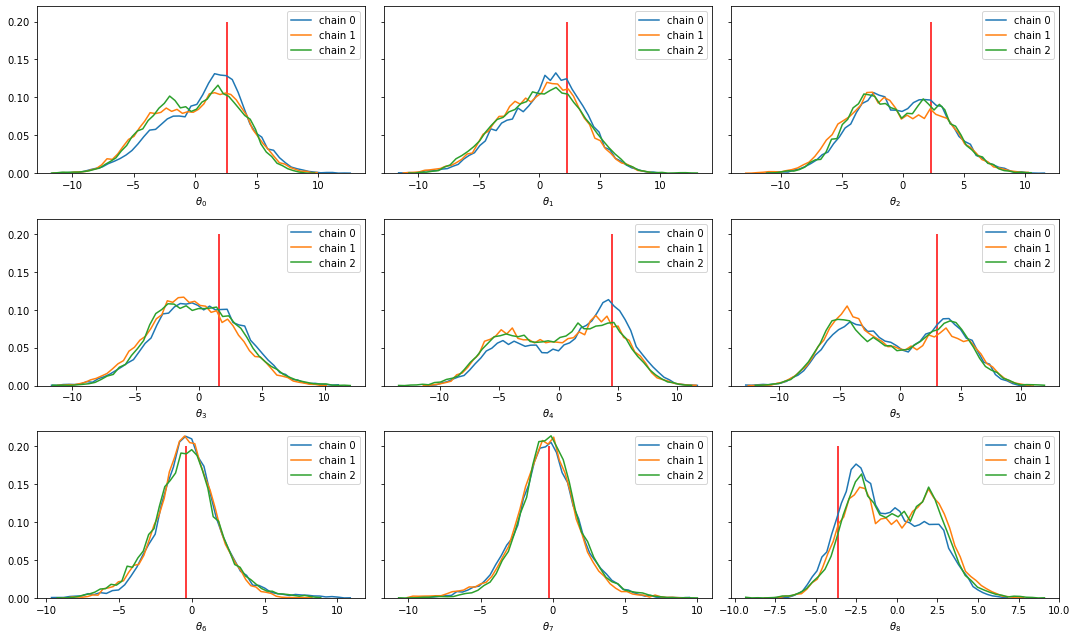
\includegraphics[width = \textwidth]{Images/marginal_dists_normprior_sc3_100k_wide_withSGD.png}
    \caption{Marginal posterior of NN with 1 hidden layer of 2 nodes}
    \label{fig:marg_post_nn2}
\end{figure}

First of all, we see that the three sparsely initialized chains of length 75,000 after a burnin of 25,000, are very similarly distributed. This is a simple visual hint that our samples gained from the Metropolis Hastings algorithm converged towards the true posterior and further reassure the results from Gelman-Rubin diagnostics.

Now let's look at the qualitative aspects of the marginal posteriors. The figure shows that while some of the parameters are distributed with one mode, some exhibit bi-modal behaviour. Furthermore, some distributions have a wide support, whereas others have a more narrow support. Since the posterior density is by definition the reciprocal of the loss, we know that areas of high posterior density is equivalent to a low loss and vice versa.
These simple observations clearly demonstrate the main motivation behind Bayesian neural networks, because it is a way to visualise the loss landscape and provides a full probabilistic framework.

We know that any frequentist method including gradient descent would eventually converge to one of the modes of the posterior. This is tested in the subsequent experiment where we compare the \textit{optimized} results from stochastic gradient descent to these distributions. However, metaphorically speaking, in a frequentist setting one walks blind folded through the loss landscape only seeing the next tiny step, not being aware of the surroundings. On the other hand, in a Bayesian setting we draw the complete loss landscape.

\subsection{Increasing Complexity}
So far the dataset and the model implemented has been quite rudimentary. Due to the inefficiency associated with running multiple Markov chains in python and the inherent computational requirements of Bayesian neural networks, it was not viable to use standard large datasets like MNIST. However, it was still possible to reaffirm the motivation of this investigation using a neural network with $3$ hidden layers and a generated classification dataset which resembles concentric circles. This network has $13$ parameters and as we can observe from the figure in the appendix \ref{fig:mcmc_circle}, there is significant disparity between the results of the Stochastic gradient descent model and the marginal distributions. To see this in more detail, we plotted the progress of the gradient descent solution, and in some cases, the solution was found to be moving \textit{away} from the mode of the distribution (figure \ref{fig:mcmc_tot}). This result is a little puzzling, since we would expect that the solution of the stochastic gradient descent will settle down into one of the modes. We checked our code very carefully and tried different sampling hyper parameters as well as different training times for gradient descent. Potentially, the actual posterior is not as smooth as the plots suggest. This could be due to number of intervals used in the plotting of the densities being too low. 

\begin{figure}[h!]
    \centering
    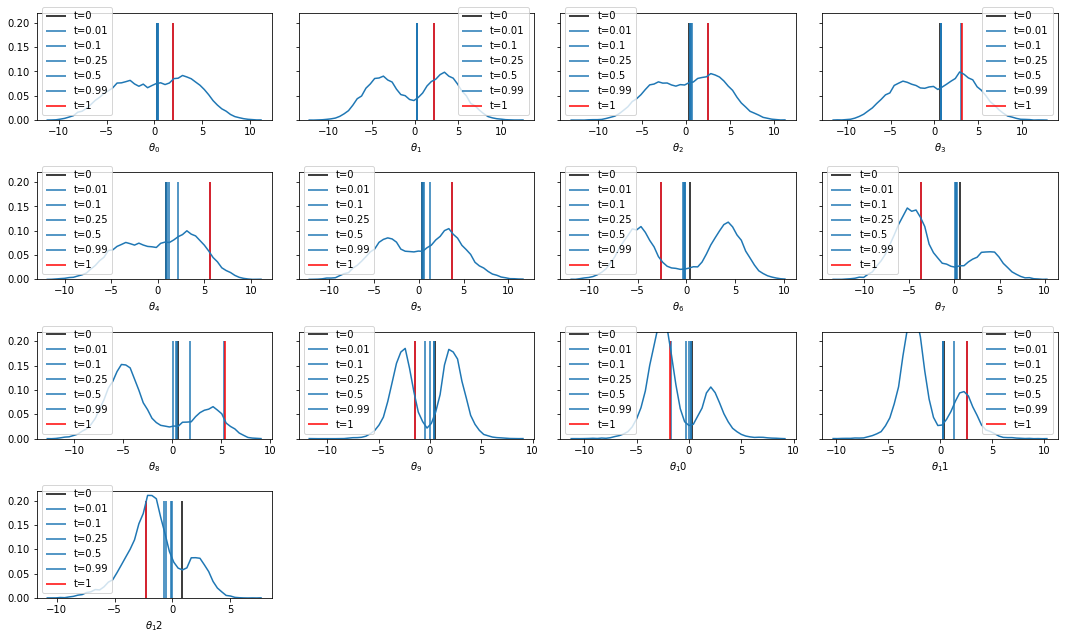
\includegraphics[width = \linewidth]{Images/mcmc_tot_circle.png}
    \caption{Sum of MCMC chains for the marginal  parameter distributions. Red vertical line corresponds to \textit{optimal} $\theta_l$}
    \label{fig:mcmc_tot}
\end{figure}

\section{Bayesian Model Averaging (BMA)}
BMA is a method for selection of models and improving estimation and prediction, which produces a model choice criteria that produces less risky predictions. If multiple models can provide adequate descriptions of the distributions, in standard frequentist neural networks only one model would be selected. All further inference is made based purely on this model. However, as we have learned, selection of one particular model can lead to inferences that ignore the existent model uncertainty. On the other hand, BMA can improve on that issue.
   
Let there be $K$ models that provide acceptable predictions of the observed data $\mathbf{Y}$. Then, $M_l, l = 1,2,...,K$ represents a set of probability distributions for the likelihood functions $L(\mathbf{Y}|\theta_l,M_l)$ in terms of model specific parameters $\theta_l$. 

The posterior distribution for the model $l$ is given by:
\begin{equation}
    \pi(\mathbf{Y}|M_l) = \int L(\mathbf{Y}|\theta_l,M_l)\pi(\theta_l|M_l)d\theta_1.
    \label{eq2}
\end{equation}
BMA assumes a prior distribution over the set of all considered models describing the prior uncertainty over each model. Given a probability mass function over all the models with values $\pi(M_l)$ for $l=1,...,K$, the posterior model probabilities are,
\begin{equation}
\label{post_prob}
    \pi(M_l|\mathbf{Y}) = \frac{\pi(\mathbf{Y}|M_l)\pi(M_l)}{\sum_{m=1}^K \pi(\mathbf{Y}|M_m)\pi(M_m)},
\end{equation}
which represents the backing of each considered model by the observed data \cite{fragoso_bayesian_2018}. The posterior probabilities can be used as a model selection criteria, with the model with the highest posterior probability being selected. However, the more \textit{Bayesian} approach would be to combine models to obtain combined parameter estimates\cite{roberts1965}. 

The next step in our numerical experiments is to incorporate BMA using the posteriors of the neural network with one hidden layer of three nodes for the circle data. There are difficulties involved in implementing BMA such as defining the prior distribution over the considered models and calculating the evidence for each model (equation \ref{eq2}) which are non trivial \cite{friel_estimating_2012}. 

In order to analyse our models, we used Bayesian Information Criterion (BIC) to estimate likelihoods for each model \cite{kaggle}. For a model $M$ with normally distributed errors, the BIC is given by,
\begin{equation}
    BIC = n \log{(\mathcal{L})} + t \log{(n)},
\end{equation}

where $n$ is the number of data points, $t$ is the number of parameters and $\mathcal{L}$ is the loss. The likelihood of the model would then be,
\begin{equation}
    L(\mathbf{Y}|\theta_l,M_l) = e^{-BIC/2}.
\end{equation}

The probability of any model $M_l$ can now be calculated from equation \ref{post_prob}. This probability can be used to calculate the expected value for any parameter $\theta_t \in \mathbf{\theta}$, which is the average value of the parameter over all models containing the parameter (in our case, all models contain all parameters), weighted by the probability of each model, i.e.,
\begin{equation}
    \mathbf{E}(\theta_t) = \frac{1}{K}\sum_l^K \pi(M_l|\mathbf{Y}) \theta_t^{(l)},
\end{equation}
where $\theta_t^{(l)}$ is the parameter $\theta_t$ in the model $M_l$.

Figure \ref{fig:bma} shows the classification of circle data with the parameters being averaged over the entire loss landscape. One of the reasons why this method performed worse in this case could be that we used BMA over all sampled $\theta$ as opposed to selecting the models that we know give acceptable results. Due to the number of models in consideration (15000), the probability for a \textit{bad} model could be lower than machine epsilon and can therefore give rise to floating point errors in the BMA calculations. Further research is warranted.
\section{Retraining the model}
\begin{figure}[!h]
		\begin{subfigure}[t]{0.5\textwidth}  
			\centering 
			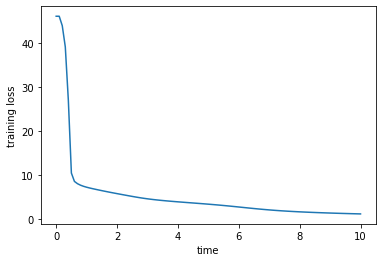
\includegraphics[width=0.9\textwidth]{Images/training_loss_bayes.png}
			\caption{Bayesian initial parameters}\label{fig:loss_b}
		\end{subfigure}%
			\begin{subfigure}[t]{0.5\textwidth}  
			\centering 
			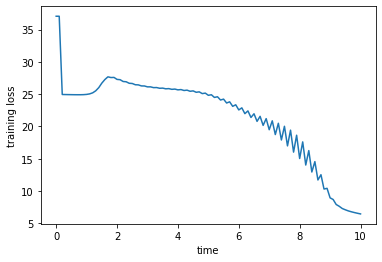
\includegraphics[width=0.9\textwidth]{Images/training_loss_gd.png}
			\caption{Random initial parameters}\label{loss_a}
		\end{subfigure}
		\label{trainingloss}
		\caption{Comparison of evolution of training loss - Bayesian v. Frequentist }
\end{figure}

Figure \ref{fig:loss_b} shows the improvement in the trajectory of the training loss when the initial parameters are chosen as the modes from the marginal distribution. In the version of the SGD model with random values for the initial parameters (\ref{loss_a}, we see that the loss hits a local minimum of approximately 25, at which point the model stops improving for a considerable amount of time. Even though it does improve afterwards, it is in start contrast with figure \ref{fig:loss_b} where the initial parameters are chosen using Bayesian inference. The loss almost immediately drops to 10 and continues to drop at a steady rate. This result opens up pathways into optimizing the training of models via Bayesian inference. 
\newline
Also of note in \ref{loss_a} is the very high initial loss at what was estimated to be the MAP of the posterior distributions. Error in this MAP estimate cannot account for this large loss since the posterior indicates that parameter values close to MAP should also perform well. One explanation could be that within the distributions we found there exist finer fluctuations that are smoothed out by our use of only 50 intervals in our histogram density plots. Greater complexity could lie beneath the posterior approximations. Further analysis would need to be carried out to establish the definitive cause of this result. 

\begin{figure}[!h]

		\hfill
		\begin{subfigure}[b]{0.325\textwidth}  
			\centering 
			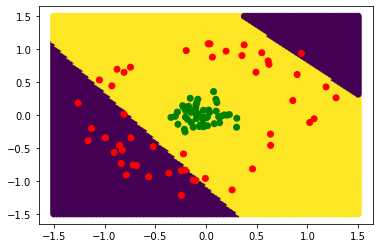
\includegraphics[width=\textwidth]{Images/gd.png}
			\caption{}
			\label{fig:gd}
		\end{subfigure}
		\hfill
			\begin{subfigure}[b]{0.325\textwidth}  
			\centering 
			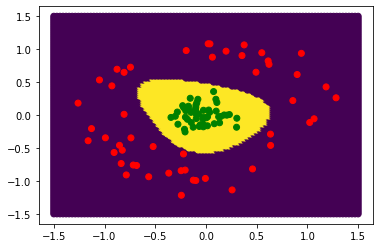
\includegraphics[width=\textwidth]{Images/mode.png}
			\caption{}
			\label{fig:mode}
		\end{subfigure}
		\hfill
		\begin{subfigure}[b]{0.325\textwidth}  
			\centering 
			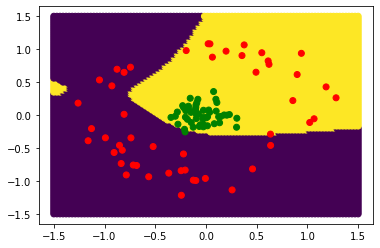
\includegraphics[width=\textwidth]{Images/bma.png}
			\caption{}
			\label{fig:bma}
		\end{subfigure}
		\caption{(a). Gradient descent with random initial parameters, (b). Gradient descent with Bayesian initial parameters, (c). Classification with Bayesian model averaged parameters.}  
		\label{fig:varying speed and length}
	\end{figure}

\section{Conclusion}
Our investigation has outlined a framework for the creation of a Bayesian neural network and has demonstrated a technique with which to sample from the posterior distributions of network parameters. Via analysis of these distributions we can provide gradient descent techniques with more more informed initial conditions which are more conducive to successful training (see \ref{fig:gd} and \ref{fig:mode}). We illustrated this by choosing the mode of our posterior for the initial parameter for gradient descent. In applying this approach to more complex networks you will likely produce more varied posterior distributions that may require more detailed analysis rather than picking the MAP of each distribution. We would suggest that such analysis should include consideration for the shape of the distributions around the modes and the corresponding shape of the loss function minima to understand potential generalisation problems (see section \ref{sec:gen_error}). \newline
We have also shown how Bayesian model averaging can be implemented to evaluate posterior distributions, however, as illustrated in \ref{fig:bma}, the model gained from BMA was not successful. Further investigation would need to take place in order to determine the lack of success achieved by BMA in this instance.

\bibliographystyle{unsrt}
\bibliography{citations.bib}

\newpage

\section*{Appendix}
Circle data
\begin{figure}[h!]
    \centering
    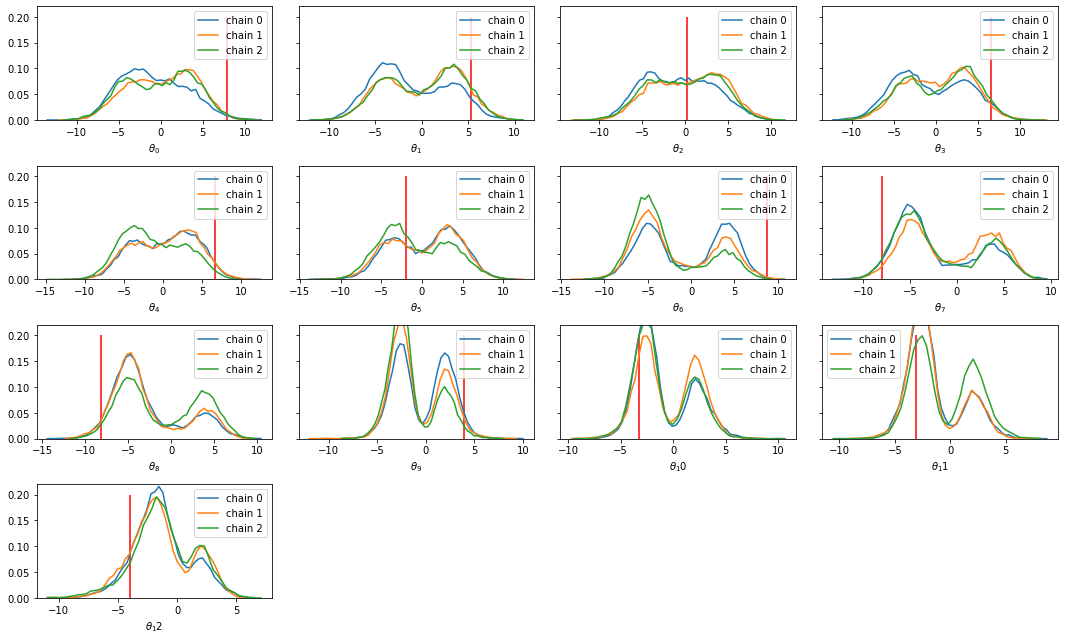
\includegraphics[width = \linewidth]{Images/marg_post_circle_nn3.png}
    \caption{The three chains of the MCMC marginal parameter distributions. Red vertical line corresponds to Gradient Descent $\theta_l$}
    \label{fig:mcmc_circle}
\end{figure}

\end{document}
